% THIS DOCUMENT IS TAILORED TO REQUIREMENTS FOR SCIENTIFIC COMPUTING.  IT SHOULDN'T
% BE USED FOR NON-SCIENTIFIC COMPUTING PROJECTS
\documentclass[12pt]{article}

\usepackage{amsmath, mathtools}
\usepackage{amsfonts}
\usepackage{amssymb}
\usepackage{graphicx}
\usepackage{colortbl}
\usepackage{xr}
\usepackage{hyperref}
\usepackage{longtable}
\usepackage{xfrac}
\usepackage{tabularx}
\usepackage{float}
\usepackage{siunitx}
\usepackage{booktabs}
\usepackage{caption}
\usepackage{pdflscape}
\usepackage{afterpage}

\usepackage[round]{natbib}

%\usepackage{refcheck}

\hypersetup{
    bookmarks=true,         % show bookmarks bar?
      colorlinks=true,       % false: boxed links; true: colored links
    linkcolor=red,          % color of internal links (change box color with linkbordercolor)
    citecolor=green,        % color of links to bibliography
    filecolor=magenta,      % color of file links
    urlcolor=cyan           % color of external links
}

%% Comments

\usepackage{color}

\newif\ifcomments\commentstrue %displays comments
%\newif\ifcomments\commentsfalse %so that comments do not display

\ifcomments
\newcommand{\authornote}[3]{\textcolor{#1}{[#3 ---#2]}}
\newcommand{\todo}[1]{\textcolor{red}{[TODO: #1]}}
\else
\newcommand{\authornote}[3]{}
\newcommand{\todo}[1]{}
\fi

\newcommand{\wss}[1]{\authornote{blue}{SS}{#1}} 
\newcommand{\plt}[1]{\authornote{magenta}{TPLT}{#1}} %For explanation of the template
\newcommand{\an}[1]{\authornote{cyan}{Author}{#1}}

%% Common Parts

\newcommand{\progname}{TTE RecSys} % PUT YOUR PROGRAM NAME HERE
\newcommand{\authname}{Yinying Huo} % AUTHOR NAMES                  

\usepackage{hyperref}
    \hypersetup{colorlinks=true, linkcolor=blue, citecolor=blue, filecolor=blue,
                urlcolor=blue, unicode=false}
    \urlstyle{same}
                                


% For easy change of table widths
\newcommand{\colZwidth}{1.0\textwidth}
\newcommand{\colAwidth}{0.13\textwidth}
\newcommand{\colBwidth}{0.82\textwidth}
\newcommand{\colCwidth}{0.1\textwidth}
\newcommand{\colDwidth}{0.05\textwidth}
\newcommand{\colEwidth}{0.8\textwidth}
\newcommand{\colFwidth}{0.17\textwidth}
\newcommand{\colGwidth}{0.5\textwidth}
\newcommand{\colHwidth}{0.28\textwidth}

% Used so that cross-references have a meaningful prefix
\newcounter{defnum} %Definition Number
\newcommand{\dthedefnum}{GD\thedefnum}
\newcommand{\dref}[1]{GD\ref{#1}}
\newcounter{datadefnum} %Datadefinition Number
\newcommand{\ddthedatadefnum}{DD\thedatadefnum}
\newcommand{\ddref}[1]{DD\ref{#1}}
\newcounter{theorynum} %Theory Number
\newcommand{\tthetheorynum}{TM\thetheorynum}
\newcommand{\tref}[1]{TM\ref{#1}}
\newcounter{tablenum} %Table Number
\newcommand{\tbthetablenum}{TB\thetablenum}
\newcommand{\tbref}[1]{TB\ref{#1}}
\newcounter{assumpnum} %Assumption Number
\newcommand{\atheassumpnum}{A\theassumpnum}
\newcommand{\aref}[1]{A\ref{#1}}
\newcounter{goalnum} %Goal Number
\newcommand{\gthegoalnum}{GS\thegoalnum}
\newcommand{\gsref}[1]{GS\ref{#1}}
\newcounter{instnum} %Instance Number
\newcommand{\itheinstnum}{IM\theinstnum}
\newcommand{\iref}[1]{IM\ref{#1}}
\newcounter{reqnum} %Requirement Number
\newcommand{\rthereqnum}{R\thereqnum}
\newcommand{\rref}[1]{R\ref{#1}}
\newcounter{nfrnum} %NFR Number
\newcommand{\rthenfrnum}{NFR\thenfrnum}
\newcommand{\nfrref}[1]{NFR\ref{#1}}
\newcounter{lcnum} %Likely change number
\newcommand{\lthelcnum}{LC\thelcnum}
\newcommand{\lcref}[1]{LC\ref{#1}}

\usepackage{fullpage}

\newcommand{\deftheory}[9][Not Applicable]
{
\newpage
\noindent \rule{\textwidth}{0.5mm}

\paragraph{RefName: } \textbf{#2} \phantomsection 
\label{#2}

\paragraph{Label:} #3

\noindent \rule{\textwidth}{0.5mm}

\paragraph{Equation:}

#4

\paragraph{Description:}

#5

\paragraph{Notes:}

#6

\paragraph{Source:}

#7

\paragraph{Ref.\ By:}

#8

\paragraph{Preconditions for \hyperref[#2]{#2}:}
\label{#2_precond}

#9

\paragraph{Derivation for \hyperref[#2]{#2}:}
\label{#2_deriv}

#1

\noindent \rule{\textwidth}{0.5mm}

}

\begin{document}

\title{Software Requirements Specification for \progname: subtitle describing software} 
\author{\authname}
\date{\today}
	
\maketitle

~\newpage

\pagenumbering{roman}

\tableofcontents

~\newpage

\section*{Revision History}

\begin{tabularx}{\textwidth}{p{3cm}p{2cm}X}
\toprule {\bf Date} & {\bf Version} & {\bf Notes}\\
\midrule
Feb 6 2025 & 1.0 & Fisrt draft\\
% Date 2 & 1.1 & Notes\\
\bottomrule
\end{tabularx}


~\newpage

\section{Reference Material}

This section records information for easy reference.

\subsection{Abbreviations and Acronyms}

\renewcommand{\arraystretch}{1.2}
\begin{tabular}{l l} 
  \toprule		
  \textbf{symbol} & \textbf{description}\\
  \midrule 
  A & Assumption\\
  DD & Data Definition\\
  GD & General Definition\\
  GS & Goal Statement\\
  IM & Instance Model\\
  LC & Likely Change\\
  PS & Physical System Description\\
  R & Requirement\\
  SRS & Software Requirements Specification\\
  \progname{} & Two-tower embending recommendation system\\
  TM & Theoretical Model\\
  DNN & Deep Neural Network\\
  ANN & Approximate Nearest Neighbor\\
  \bottomrule
\end{tabular}\\


\subsection{Mathematical Notation}

\renewcommand{\arraystretch}{1.2}
\begin{tabular}{l l} 
  \toprule		
  \textbf{symbol} & \textbf{description}\\
  \midrule 
  $\mathbb{R}$ & Real number\\
  $\theta$ & model parameter,a vector of real numbers\\
  $u(\cdot)$ & A function that map model parameter $\theta$ and features of user to the embedding space.\\
  $v(\cdot)$ & A function that map model parameter $\theta $ and features of item to the embedding space.\\
  $x_i$ & user feature\\
  $y_i$ & item feature\\
  $r_i$ & the associated reward for each user and item pair\\ 
  $J(\cdot)$ & regularization function to prevent overfitting\\
  $\mathcal{L}(\theta)$ & Loss function\\
  $\eta $ & learning rate\\
  $B $ & mini-batch\\
  \bottomrule
\end{tabular}\\

\section{Introduction}
In the digital era, recommendation systems play a crucial role in enhancing user experiences by providing personalized content, products, and services. These systems are widely used in industries such as e-commerce, streaming platforms, and social media to help users discover relevant items from vast catalogs. Traditional recommendation approaches, including collaborative filtering and content-based methods, rely on explicit user-item interactions or manually engineered features. However, as datasets grow in complexity and size, these methods face challenges in scalability and efficiency.

To overcome these limitations, modern recommendation systems leverage deep learning-based techniques, such as Two-Tower Embeddings (TTE). This project implements a recommendation system using a TTE model, where user and item features are mapped into a shared embedding space. To efficiently retrieve relevant items, Approximate Nearest Neighbors (ANN) search with FAISS is used for candidate selection, followed by dot product similarity for ranking.

The training dataset used for this project is from Kaggle: \url{https://www.kaggle.com/datasets/arashnic/book-recommendation-dataset}.

\subsection{Purpose of Document}

The purpose of this document is to define the software requirements for the recommendation system based on Two-Tower Embeddings (TTE). It serves as a reference for the system’s functionality, design considerations, and constraints.

\subsection{Scope of Requirements} 

This project assumes that users and items are fully represented by the features available in the dataset. External factors, such as social influences, or temporal patterns, are not considered. The recommendation model will rely solely on the provided user-item interaction data to generate recommendations.

\subsection{Characteristics of Intended Reader} \label{sec_IntendedReader}
Readers of this documentation are expected to have completed an introductory course on machine learning.

\subsection{Organization of Document}

This document starts with reference materials, such as abbreviations and mathematical notation, followed by the problem, objectives, assumptions, theoretical model, and instance models. It also defines the project's functional and nonfunctional requirements.

\section{General System Description}

This section provides general information about the system.  It identifies the
interfaces between the system and its environment, describes the user
characteristics and lists the system constraints. 

\subsection{System Context}

\begin{figure}[h!]
\begin{center}
 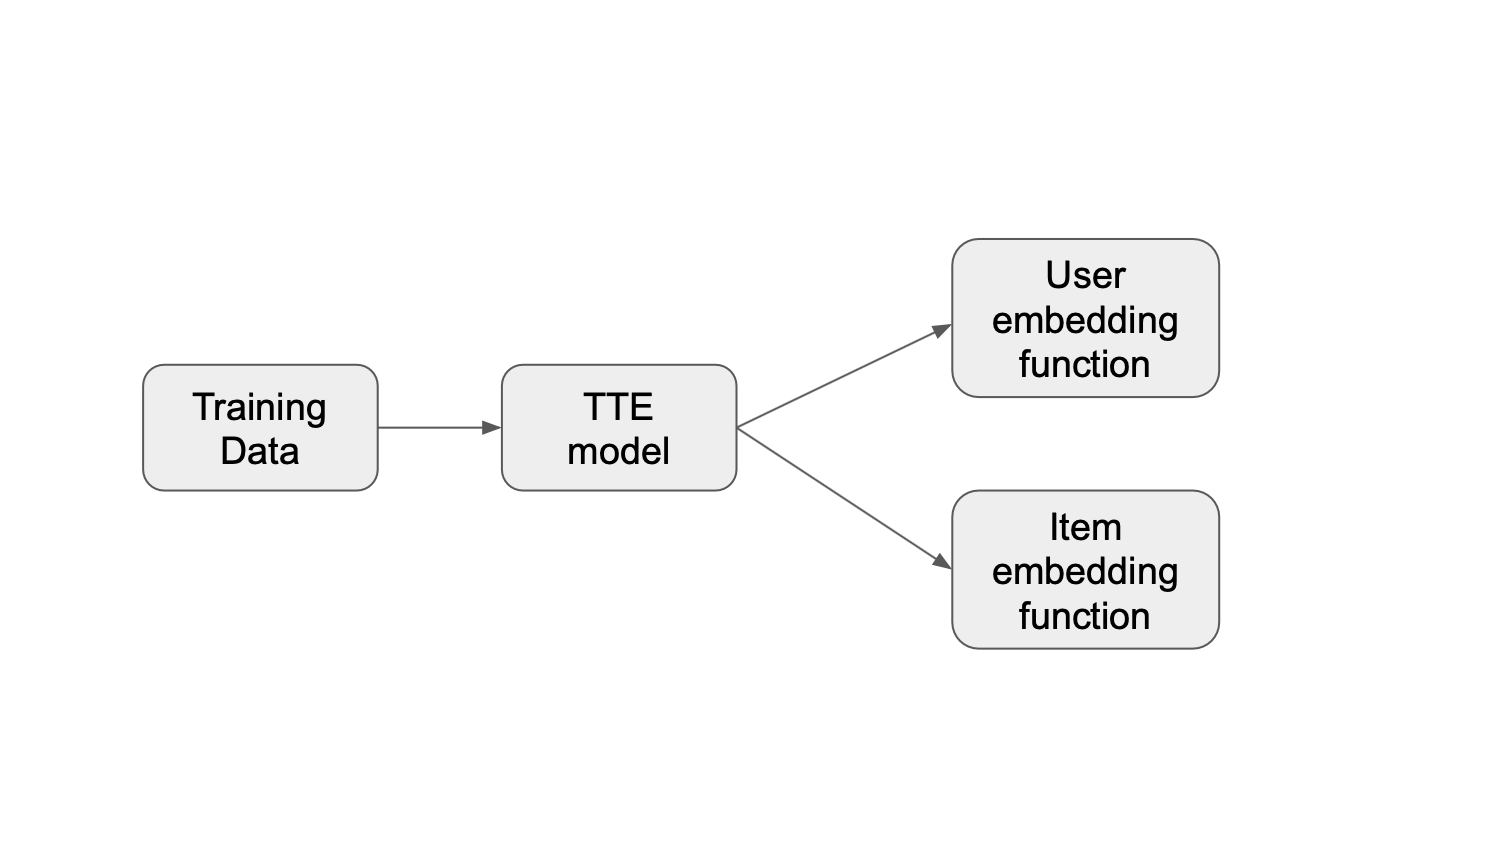
\includegraphics[width=0.6\textwidth]{image1}
\caption{Training phase}
\label{Fig_SystemContext1} 
\end{center}

\end{figure}
\begin{figure}[h!]
  \begin{center}
   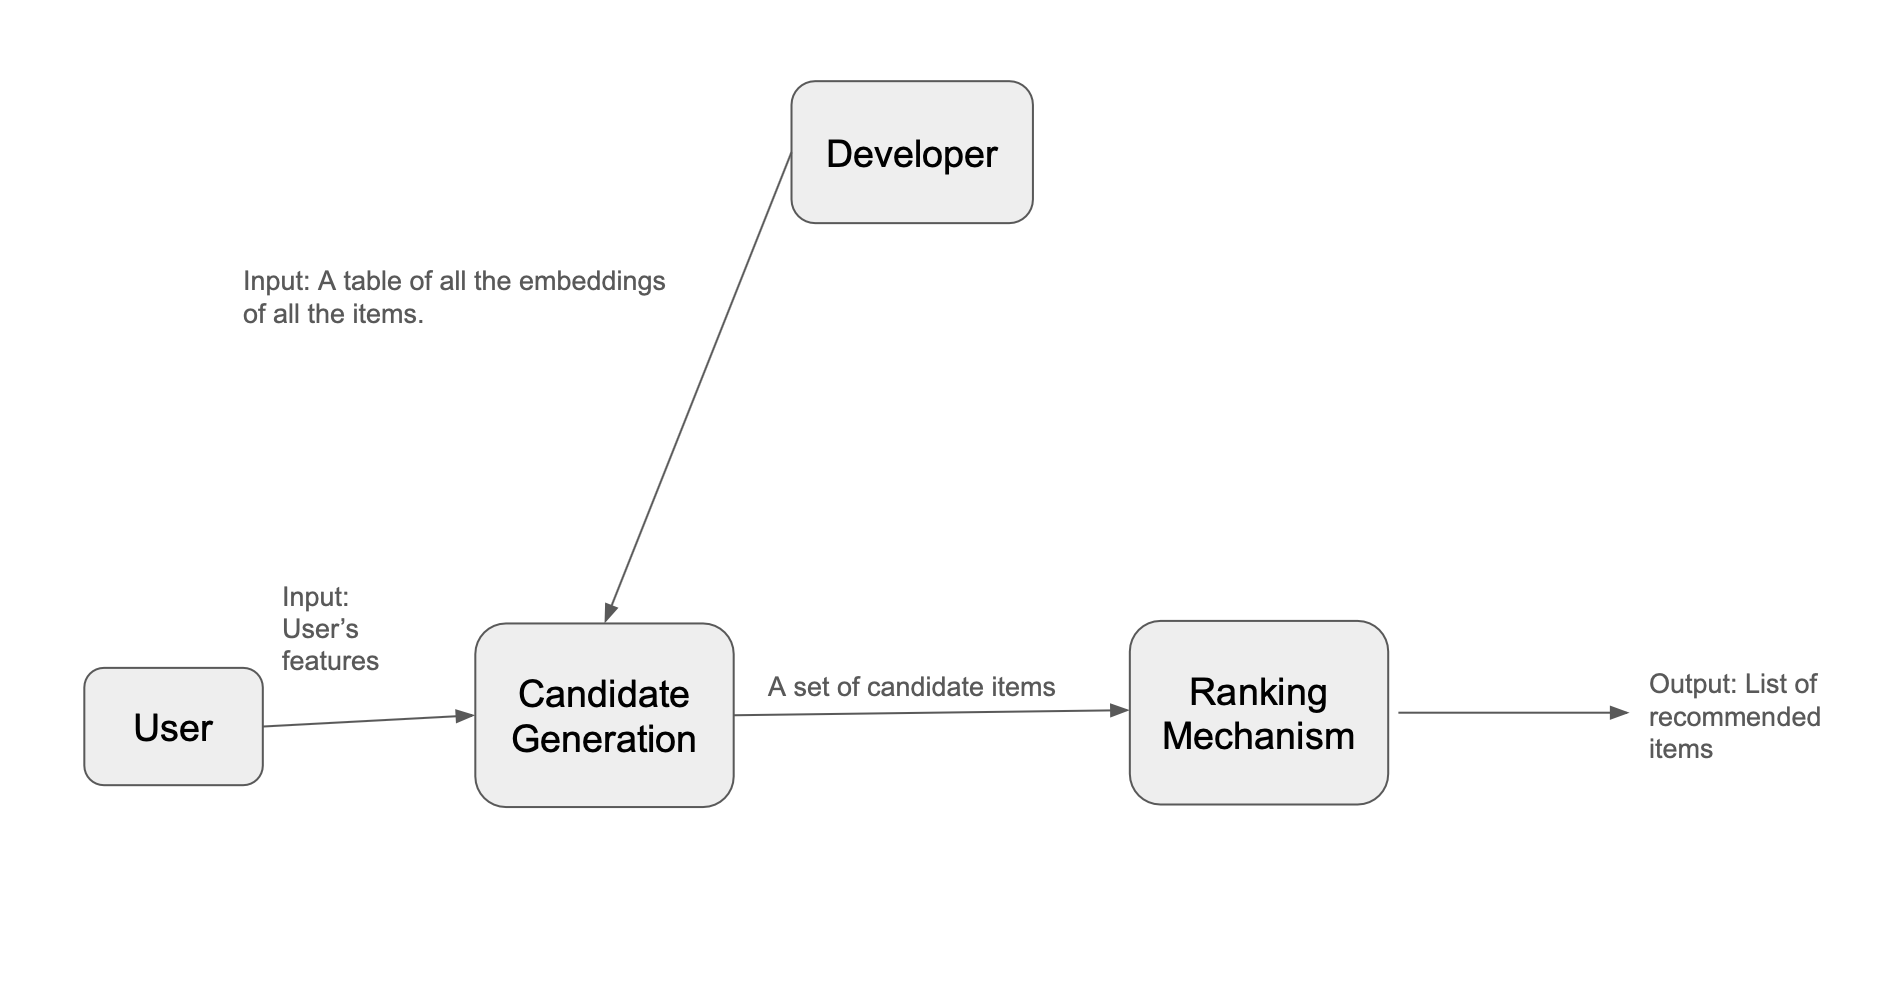
\includegraphics[width=0.9\textwidth]{image2}
  \caption{Inference phase}
  \label{Fig_SystemContext2} 
  \end{center}
  \end{figure}
The recommendation system follows a structured workflow consisting of two main phases: \textbf{training} and \textbf{inference}. The system leverages Two-Tower Embeddings and ANN search to generate personalized recommendations efficiently.

Training Phase

During the training phase, the system learns two embedding functions:

\begin{itemize}
    \item \textbf{User Embedding Function:} Maps user features (e.g., age=20, gender=male) into a fixed-dimensional vector representation (e.g., $[1,2.3,4]$) in the embedding space.
    \item \textbf{Item Embedding Function:} Maps item features into the same embedding space as users.
\end{itemize}
During the training phase, the objective is to make the dot product of the outputs of the two embedding functions approximately equal to the associated rating $r_i$. This can be achieved by minimizing the loss function.

Once training is complete, the item embedding function is used to precompute embeddings for all items. These embeddings are stored in an ANN index for efficient retrieval during inference.

Inference Phase

When a user interacts with the system, the following steps occur:

\begin{enumerate}
    \item The user's features are processed by the user embedding function to generate an embedding.
    \item This embedding is used as a query in the ANN index to retrieve a set of candidate items.
    \item Candidates are ranked by similarity (via dot product).
    \item The final ranked list is presented as recommendations to the user.
\end{enumerate}

\begin{itemize}
  \item User Responsibilities:
  \begin{itemize}
  \item Provide correct inputs.
  \end{itemize}
  \item Developer Responsibilities:
  \begin{itemize}
  \item Precompute item embeddings before the user interacts with the system.
  \end{itemize}
  \item \progname{} Responsibilities:
  \begin{itemize}
  \item Detect data type mismatches.
  \item Generate recommendations as output.
  \end{itemize}
\end{itemize}
  

\subsection{User Characteristics} \label{SecUserCharacteristics}

The end user are not required to have any technical knowledge. The only responsibility of the user is to provide their information in the required format.

\subsection{System Constraints}

There is no system constrains for this software.

\section{Specific System Description}

This section first presents the problem description, which gives a high-level
view of the problem to be solved.  This is followed by the solution characteristics
specification, which presents the assumptions, theories, definitions and finally
the instance models. 

\subsection{Problem Description} \label{Sec_pd}

\progname{} is intended to build a recommendation system based on the Two-Tower Embeddings architecture.


\subsubsection{Terminology and  Definitions}

This subsection provides a list of terms that are used in the subsequent
sections and their meaning, with the purpose of reducing ambiguity and making it
easier to correctly understand the requirements:

\begin{itemize}

  \item \textbf{Approximate Nearest Neighbor (ANN) Search}: A method for efficiently retrieving the most similar items to a query embedding by approximating the nearest neighbor search
  \item \textbf{Embedding}: A dense, low-dimensional vector representation of a user or item in a continuous vector space. Embeddings capture semantic relationships and are learned by the two-tower model.
  \item \textbf{Two-Tower Embedding (Model)}: A neural network architecture consisting of two separate towers (user and item) that generate embeddings. The model is trained to predict user-item relevance.
  \item \textbf{Regularization}: A technique to prevent overfitting by adding a penalty term to the loss function.
  \item  \textbf{Batch}: A subset of the training dataset used during a single optimization step.

\end{itemize}

\subsubsection{Goal Statements}


\begin{itemize}

\item[GS\refstepcounter{goalnum}\thegoalnum \label{GS1}:] Learn the embedding functions from a training dataset.
\item[GS\refstepcounter{goalnum}\thegoalnum \label{GS2}:] Return a list of recommended items.
\end{itemize}


\subsection{Solution Characteristics Specification}

\subsubsection{Modelling Decisions}

This project will be written in Python due to the availability of various machine learning libraries in Python.

\subsubsection{Assumptions} \label{sec_assumpt}

This section simplifies the original problem and helps in developing the
theoretical model by filling in the missing information for the physical system.
The numbers given in the square brackets refer to the theoretical model [TM],
general definition [GD], instance model [IM], or likely
change [LC], in which the respective assumption is used.

\begin{itemize}

\item[A\refstepcounter{assumpnum}\theassumpnum \label{A_Embedding1}:]
User features can be effectively represented as low-dimensional dense vectors (embeddings). [IM1][IM2][IM3][LC1]

\item[A\refstepcounter{assumpnum}\theassumpnum \label{A_Embedding2}:]
Item features can be effectively represented as low-dimensional dense vectors (embeddings). [IM1][IM2][IM3][LC1]


\item[A\refstepcounter{assumpnum}\theassumpnum \label{A_DotProduct}:]
The dot product between user and item embeddings is a valid measure of user interest in items. [IM1][IM2][IM3]

\item[A\refstepcounter{assumpnum}\theassumpnum \label{A_DataQuality}:]
User-item interactions in the training data reflect true user preferences and are free from systemic bias. [IM1][IM2][IM3]

\end{itemize}


\subsubsection{Theoretical Models}\label{sec_theoretical}

This section focuses on the general equations and laws that \progname{} is based
on. 

~\newline

\deftheory
{TM:Mean Squared Error}
{Regularized Mean Squared Error (MSE) Loss}
{
  $\displaystyle \mathcal{L}(\theta)=\min_{\theta} \frac{1}{|B|} \sum_{(x_i, y_i, r_i) \in B} \left(r_i - \langle u(x_i; \theta), v(y_i; \theta) \rangle \right)^2 + \gamma \left[ J(u) + J(v) \right]$
}
{
  The two-tower model is trained to minimize the Mean Squared Error (MSE) between predicted relevance scores $\langle u(x_i; \theta), v(y_i; \theta) \rangle$ and observed rewards $r_i$. The regularization term $\gamma \left[ J(u) + J(v) \right]$ penalizes model complexity using $L_1$ or $L_2$ norms to prevent overfitting.
}
{
  - $u(x_i; \theta), v(y_i; \theta)$: User and item embeddings generated by deep neural networks.  
  - $J(u) = \|\theta_u\|_p$, $J(v) = \|\theta_v\|_p$: Regularization on network parameters ($p=1$ or $2$).  
  - $\gamma$: Hyperparameter controlling regularization strength.  
}
{
  \url{https://en.wikipedia.org/wiki/Mean_squared_error}
}
{
  \gsref{GS1}, \aref{A_Embedding1}, \aref{A_Embedding2}
}
{
  Training batch $B \subset \mathcal{T}$ is sampled uniformly from the dataset.
}
{}

\deftheory
{TM:GD}
{Gradient Descent}
{
  $\displaystyle \theta_{t+1} = \theta_t - \eta \nabla_\theta \mathcal{L}(\theta_t)$
}
{
  Iterative optimization algorithm for minimizing a loss function $\mathcal{L}(\theta)$ by updating parameters $\theta$ in the direction of steepest descent.
}
{
  $\eta$: Learning rate (step size)\\
  Requires differentiable loss function\\
  Converges to local minimum
}
{
  \url{https://en.wikipedia.org/wiki/Gradient_descent}
}
{
  \iref{IM_SGD}
}
{
  $\mathcal{L}(\theta)$ must be differentiable
}
{}

~\newline

\subsubsection{Instance Models} \label{sec_instance}    

This section transforms the problem defined in Section~\ref{Sec_pd} into 
one which is expressed in mathematical terms. 

The goals \gsref{GS1} and \gsref{GS2} are addressed by the following mathematical models:

~\newline

%Instance Model 1

  \begin{minipage}{\textwidth}
    \renewcommand*{\arraystretch}{1.5}
    \begin{tabular}{| p{0.15\textwidth} | p{0.8\textwidth}|}
      \hline
      \rowcolor[gray]{0.9}
      Number& IM\refstepcounter{instnum}\theinstnum \label{IM_CandidateGen}\\
      \hline
      Label& \bf ANN-based Candidate Generation\\
      \hline
      Input& 
      \begin{itemize}
        \item User embedding $u(x_i;\theta) \in \mathbb{R}^k$ (from user tower).
        \item Precomputed item embeddings $\{v(y_i;\theta)\}_{i=1}^N \in \mathbb{R}^k$ (from item tower).
      \end{itemize}\\
      \hline
      Output& Top-$K$ candidate indices $I \subset \{1, \dots, N\}$\\
      \hline
      Description& 
      \begin{itemize}
        \item Builds an ANN index (e.g., FAISS-IVFPQ) over $\{v(y_i;\theta)\}_{i=1}^N$.
        \item Queries the index with $\mathbf{u}_\theta$ to retrieve candidates: 
          $I = \text{ANN-Search}\left(v(y_i;\theta), \{v(y_i;\theta)\}_{i=1}^N, K\right)$
      \end{itemize}\\
      \hline
      Sources& \cite{douze2024faisslibrary}\\
      \hline
      Ref.\ By & \rref{R_VerifyOutput}, \rref{R_Output}, \gsref{GS2}\\
      \hline
    \end{tabular}
    \end{minipage}

    \begin{minipage}{\textwidth}
      \renewcommand*{\arraystretch}{1.5}
      \begin{tabular}{| p{0.15\textwidth} | p{0.8\textwidth}|}
        \hline
        \rowcolor[gray]{0.9}
        Number& IM\refstepcounter{instnum}\theinstnum \label{IM_Ranking}\\
        \hline
        Label& \bf Dot Product Ranking\\
        \hline
        Input& 
        \begin{itemize}
          \item User embedding $u(x_i;\theta)$.
          \item Candidate item embeddings $\{v(y_i;\theta)\}_{i \in I}$.
        \end{itemize}\\
        \hline
        Output& Ranked list $I_{\text{ranked}}$ sorted by $s(x_i,y_i) = \langle u(x_i;\theta),v(y_i;\theta) \rangle $.\\
        \hline
        Description&
        \begin{itemize}
          \item Computes exact dot product scores: $s(x_i,y_i) = \langle u(x_i;\theta),v(y_i;\theta) \rangle$.
          \item Sorts candidates in descending order of $s(x_i,y_i)$.
          \item Returns top-$N$ items: $I_{\text{ranked}} = \text{argsort}(s_i)[:N]$.
        \end{itemize}\\
        \hline
        Sources& \url{https://en.wikipedia.org/wiki/Dot_product}\\
        \hline
        Ref.\ By & \rref{R_VerifyOutput}, \rref{R_Output}, \gsref{GS2}\\
        \hline
      \end{tabular}
      \end{minipage}
%~\newline
\begin{minipage}{\textwidth}
  \renewcommand*{\arraystretch}{1.5}
  \begin{tabular}{| p{0.15\textwidth} | p{0.8\textwidth}|}
  \hline
  \rowcolor[gray]{0.9}
  Number& IM\refstepcounter{instnum}\theinstnum \label{IM_SGD}\\
  \hline
  Label& \bf Stochastic Gradient Descent\\
  \hline
  Input& 
  \begin{itemize}
    \item Training dataset $\mathcal{D} = \{(x_i, y_i, r_i)\}_{i=1}^T$
    \item Initial parameters $\theta_0$
    \item Learning rate $\eta$
    \item Mini-batch size $|B|$
  \end{itemize}\\
  \hline
  Output& Learned parameters $\theta^*$\\
  \hline
  Description&
  \begin{itemize}
    \item For each iteration:
      \begin{enumerate}
        \item Sample mini-batch $B \subset \mathcal{D}$
        \item Compute gradient estimate: $\nabla_\theta \mathcal{L}_B(\theta_t)$
        \item Update parameters: $\theta_{t+1} = \theta_t - \eta \nabla_\theta \mathcal{L}_B(\theta_t)$
      \end{enumerate}
    \item Loss function with regularization:
      $\mathcal{L}_B(\theta) = \frac{1}{|B|}\sum_{(x_i,y_i)\in B}(r_i - \langle u(x_i;\theta),v(y_i;\theta)\rangle)^2 + \gamma(J(u) - J(v))$
  \end{itemize}\\
  \hline
  Sources& \url{https://en.wikipedia.org/wiki/Stochastic_gradient_descent} \\
  \hline
  Ref.\ By &  \gsref{GS1}\\
  \hline
  \end{tabular}
  \end{minipage}

\subsubsection{Input Data Constraints} \label{sec_DataConstraints}    


\begin{table}[!h]
  \caption{Input Variables} \label{TblInputVar}
  \renewcommand{\arraystretch}{1.2}
\noindent \begin{longtable*}{l l l l c} 
  \toprule
  \textbf{Var} & \textbf{Physical Constraints} & \textbf{Software Constraints} &
                             \textbf{Typical Value} & \textbf{Uncertainty}\\
  \midrule 
  $r_i$ & $r_i \in \mathbb{R}$ & $0 \leq r_i \leq 10$ & 8  & 0\%
  \\
  \bottomrule
\end{longtable*}
\end{table}

\noindent 
\begin{description}
\item[(*)] $r_i$ is the rating that user $x_i$ assigns to the item $y_i$.
\end{description}


\section{Requirements}

This section provides the functional requirements, the business tasks that the
software is expected to complete, and the nonfunctional requirements, the
qualities that the software is expected to exhibit.

\subsection{Functional Requirements}

\noindent \begin{itemize}

\item[R\refstepcounter{reqnum}\thereqnum \label{R_Inputs}:] The system shall accept user features, item features, and training data with observed rewards.

\item[R\refstepcounter{reqnum}\thereqnum \label{R_VerifyOutput}:]
Identical user/item embeddings shall produce identical rankings.

\item[R\refstepcounter{reqnum}\thereqnum \label{R_Output}:]  The system shall return a ranked list of recommended items with similarity scores.

\end{itemize}

\subsection{Nonfunctional Requirements}

\noindent \begin{itemize}

\item[NFR\refstepcounter{nfrnum}\thenfrnum \label{NFR_Scalability}:]
  \textbf{Scalability} The system shall support incremental updates to trained models when new data becomes available, with updates completing within a time proportional to the dataset size.

\item[NFR\refstepcounter{nfrnum}\thenfrnum \label{NFR_DataPortability}:]
  \textbf{Data Portability} The system shall allow seamless replacement of datasets with different schemas or formats, requiring only configuration changes.

\item[NFR\refstepcounter{nfrnum}\thenfrnum \label{NFR_Portability}:]
  \textbf{Portability} \progname{} shall operate on Windows, Linux, and macOS environments

\end{itemize}

\subsection{Rationale}

The scope requirements are designed to simplify the model architecture and reduce computational complexity.

Assumptions \aref{A_Embedding1} and \aref{A_Embedding2} strike a balance between expressiveness and computational efficiency. Additionally, \aref{A_DotProduct} eliminates the need for normalization, preserving magnitude information in embeddings. Furthermore, \aref{A_DataQuality} ensures that the model learns meaningful patterns.

Modeling Decision Rationale: 
Python is chosen for its extensive machine learning ecosystem, including libraries such as PyTorch and FAISS, as well as its rapid prototyping capabilities and strong community support.

\section{Likely Changes}    

\noindent \begin{itemize}

\item[LC\refstepcounter{lcnum}\thelcnum\label{LC_advancedANN}:] The system may adopt more advanced ANN algorithms (e.g., ScaNN or HNSW) to improve retrieval efficiency or accuracy.

\end{itemize}

\section{Unlikely Changes}    

\noindent None



\section{Traceability Matrices and Graphs}

The purpose of the traceability matrices is to provide easy references on what
has to be additionally modified if a certain component is changed.  Every time a
component is changed, the items in the column of that component that are marked
with an ``X'' may have to be modified as well.  Table~\ref{Table:trace} shows the
dependencies of theoretical models, general definitions, data definitions, and
instance models with each other. Table~\ref{Table:R_trace} shows the
dependencies of instance models, requirements, and data constraints on each
other. Table~\ref{Table:A_trace} shows the dependencies of theoretical models,
general definitions, data definitions, instance models, and likely changes on
the assumptions.

\begin{table}[h!]
\centering
\begin{tabular}{|c|c|c|c|c|c|}
\hline
	& \aref{A_Embedding1}& \aref{A_Embedding2}& \aref{A_DotProduct}& \aref{A_DataQuality}  \\
\hline
\tref{TM:GD}          & X&X & & \\ \hline
\tref{TM:Mean Squared Error}          & &  &X &X\\ \hline
\iref{IM_CandidateGen}         & X& X & X&X \\ \hline
\iref{IM_Ranking}         & X& X &X & X\\ \hline
\iref{IM_SGD}         & X&X & & \\ \hline
\lcref{LC_advancedANN}      & X & X & &X\\ \hline

\hline
\end{tabular}
\caption{Traceability Matrix Showing the Connections Between Assumptions and Other Items}
\label{Table:A_trace}
\end{table}


\begin{table}[h!]
\centering
\begin{tabular}{|c|c|c|}
\hline        
	& \tref{TM:GD}& \tref{TM:Mean Squared Error} \\
\hline
\iref{IM_SGD}     & X& X   \\ \hline
\iref{IM_Ranking}        & & X \\ \hline
\iref{IM_CandidateGen}      &  &X   \\ \hline

\end{tabular}
\caption{Traceability Matrix Showing the Connections Between Items of Different Sections}
\label{Table:trace}
\end{table}

\begin{table}[h!]
\centering
\begin{tabular}{|c|c|c|c|}
\hline
	& \iref{IM_CandidateGen}& \iref{IM_Ranking}& \iref{IM_SGD}\\
\hline
\rref{R_Inputs}     & X& &     \\ \hline
\rref{R_VerifyOutput}    & &  X &    \\ \hline
\rref{R_Output}   & X& X& X    \\ \hline


\end{tabular}
\caption{Traceability Matrix Showing the Connections Between Requirements and Instance Models}
\label{Table:R_trace}
\end{table}

\bibliographystyle {plainnat}
\bibliography {../../refs/References}

\end{document}